\chapter{Streams \& I/O}

\section{Files}

We turn our computers on and off. The contents of its main memory are transient, and depend 
on the power supply. So when we turn it off, we lose all the data that was in memory. Some data
needs to be stored permanently, so that we can access it later. This is where files come in.
A \textbf{file} is a sequence of bytes stored on a permanent storage device, such as a hard disk.
Files are used to store data permanently, and to share data between different programs. A file 
has a name, and the data that is in it is stored in a specific format. We can read and 
write on a file if we know its name and its format. \\

At a fundamental level, a file is a sequence of bytes numbered from 0 to $n-1$, where $n$ is the
size of the file in bytes. Other notions can be supplied by programs that interpret a file format.
For example, the 6 bytes corresponding to "123.45" might be interpreted as the floating-point
number 123.45. \\

To \textbf{read} a file:
\begin{itemize}
    \item We must know its name.
    \item We must open it (for reading).
    \item Then we can read it.
    \item Once finished, we must close it:
    \begin{itemize}
        \item That is typically done implicitly (when the stream object is destroyed).
    \end{itemize}
\end{itemize}

To \textbf{write} a file:
\begin{itemize}
    \item We must name it
    \item We must open it (for writing), or create a new file of that name.
    \item Then we can write to it.
    \item Once finished, we must close it.
    \begin{itemize}
        \item That is typically done implicitly (when the stream object is destroyed).
    \end{itemize}
\end{itemize}

\subsection{Opening and closing files}

To open a file, we use 2 main objects: \texttt{ifstream} and \texttt{ofstream}. The former is used
to read from a file, and the latter is used to write to a file. Both are defined in the \texttt{fstream}
header. \\

For example, to open a file for reading:\\

\begin{lstlisting}[language=C++]
#include <fstream>

int main() {
    cout << "Please enter the name of the file you want to read: ";
    string filename;
    cin >> filename;

    ifstream ist{filename};

    if (!ist) {
        cerr << "Can't open input file " << filename << endl;
        return 1;
    }
}
\end{lstlisting}

To open a file for writing:\\

\begin{lstlisting}[language=C++]
int main() {
    cout << "Please enter the name of the file you want to write to: ";
    string filename;
    cin >> filename;

    ofstream ost{filename};

    if (!ost) {
        cerr << "Can't open output file " << filename << endl;
        return 1;
    }
}
\end{lstlisting}

To close a file, we can use the \texttt{close()} method. However, this is not necessary, as the 
file will be closed automatically when the stream object is destroyed. This happens when the
stream object goes out of scope. For example:\\

\begin{lstlisting}[language=C++]
if(read) {
    ifstream input{filename};

    if (input) {
        process(input);
    } else {
        cerr << "Can't open input file " << filename << endl;
        return 1;
    }

} // input goes out of scope, and the file is closed
\end{lstlisting}

\subsection{Reading from a file}

To read from a file, we can use the \texttt{>>} operator. For example, suppose that a file
contains a sequence of pairs represanting hours and temperature readings, like this:\\

\begin{lstlisting}[language=C++]
10 20.5
11 21.3
12 22.1
\end{lstlisting}

The hours are numbered from 0 to 23, and the temperatures are floating-point numbers. No further
information is assumed, and when we reach end-of-file, or read an unexepected value, we stop.
We can read this file like this:\\

\begin{lstlisting}[language=C++]
struct Reading {
    int hour;
    double temperature;
}

vector<Reading> temps;

int hour;
double temperature;
ifstream ist{fname};

while (ist >> hour >> temperature) {
    if (hour < 0 || 23 < hour) {
        cout << "hour out of range" << endl;
    }
    temps.push_back(Reading{hour, temperature});
}
\end{lstlisting}

\subsection{No copy or assign for I/O objects}

We cannot copy or assign objects of the IO types:\\

\begin{lstlisting}[language=C++]
ofstream out1, out2;
out1 = out2; // ERROR: cannot assign stream objects

ofstream print(ofstream); // ERROR: can't initialize the ofstream parameter
out2 = print(out2); // ERROR: cannot copy stream objects
\end{lstlisting}

Because we can't copy the IO types, we cannot have a parameter of return type that is one of
the stream types. Functions that do IO typically pass and return the stream through 
\textbf{references}. Reading or writing an IO object changes its state, so the reference
\textbf{must not be const}.

\section{File modes and binary I/O}

By default, an \texttt{ifstream} opens its file for reading, and an \texttt{ofstream} opens
its file for writing. We can modify the mode in which a file is opened. The alternatives are:

\begin{itemize}
    \item \texttt{ios\_base::app}: Append, output adds to the end of the file.
    \item \texttt{ios\_base::ate}: At end, open and seek to the end.
    \item \texttt{ios\_base::binary}: Binary mode - beware of system specific behavior.
    \item \texttt{ios\_base::in}: For reading.
    \item \texttt{ios\_base::out}: For writing.
    \item \texttt{ios\_base::trunc}: Truncate file to 0-length
\end{itemize}

We can optionally specify a file mode after the name of the file:\\

\begin{lstlisting}[language=C++]
ofstream of1 {name1}; // defaults to ios_base::out
ifstream if1 {name2}; // defaults to ios_base::in
ofstream ofs {name, ios_base::app}; // append rather than overwrite
fstream fs {name, ios_base::in | ios_base::out}; // both in and out
\end{lstlisting}

\subsection{Text vs binary files}

When we read a file in binary mode, the data is read exactly as it is stored in the file, 
byte by byte. This is different from text mode, where certain translations may occur, such 
as converting newline characters to the appropriate format for the operating system (e.g., 
\verb|\n| to \verb|\r\n| on Windows).\\

In binary mode, no such translations occur, which makes it suitable for reading and writing 
non-text data, such as images, audio files, or any other format where the exact byte 
representation is crucial.

\begin{figure}[H]
    \centering
    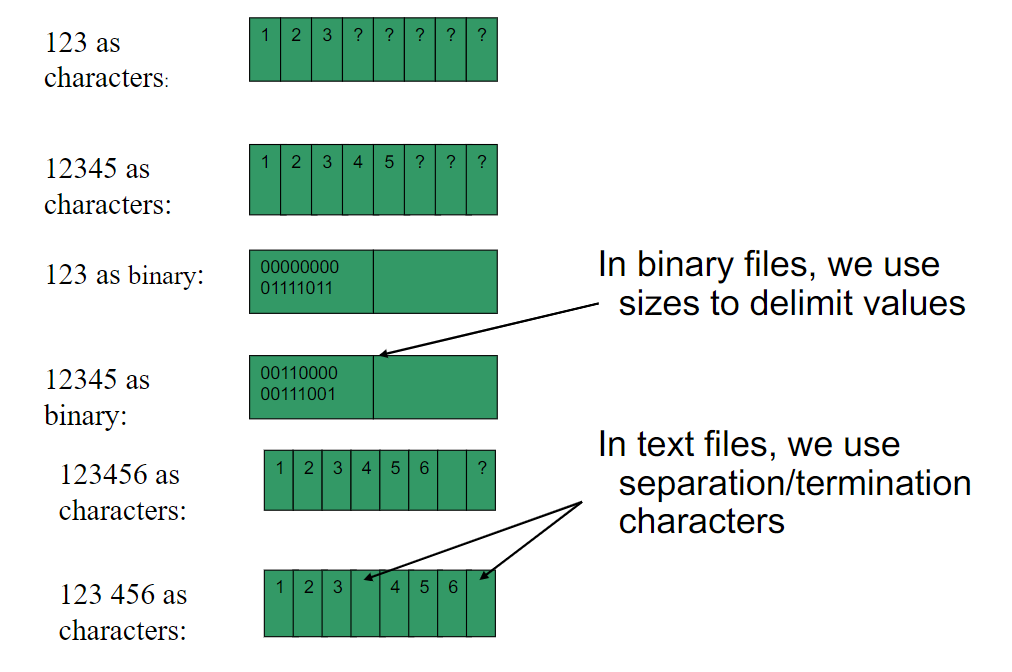
\includegraphics[width=10cm]{figures/binary_vs_text.png}
    \caption{Binary vs text reading}
    \label{fig:binary_vs_text}
\end{figure}

In the end, we should use text when we can, as we can read it without a fancy program, we can debug
more easily, it is portable across different systems, and most information can be represented 
reasonably as text. We only use binary when we must, for example, when reading image or sound files. 

\section{String streams}

A \textbf{stringstream} reads/writes from/to a \textbf{string} rather than a file or a 
keyboard/screen. For example:\\

\begin{lstlisting}[language=C++]
double str_to_double(string s) {
    istringstream is {s};

    double d;
    is >> d;
    if (!is) error("double format error: ", s);
    return d;
}

double d1 = str_to_double("12.4");
double d2 = str_to_double("1.34e-3");
double d3 = str_to_double("twelve point three"); // ERROR
\end{lstlisting}

String streams are very useful for:
\begin{itemize}
    \item Formatting into a fixed-sized space (think GUI)
    \item For extracting typed objects out of a string.
\end{itemize}

\subsection{Type vs line}

How to read a string:

\begin{lstlisting}[language=C++]
string name;
cin >> name;          // input: Dennis Ritchie
cout << name << '\n'; // output: Dennis
\end{lstlisting}

How to read a line:

\begin{lstlisting}[language=C++]
string name;
getline(cin, name);   \\ input: Dennis Ritchie
cout << name << '\n'; \\ output Dennis Ritchie

\\ Now what? Maybe:
istringstream ss{name};
ss >> first_name;
ss >> second_name;
\end{lstlisting}

\section{Examples}

\subsection{Reading a \texttt{.csv} file}

An \texttt{istringstream} is often used when we have some work to do on an entire line, and other
work to do with individual words within a line.\\

For example, when opening a \texttt{.csv} file, we want to read each line, and do some tasks with
the information within each line of the file:\\

\begin{lstlisting}[language=C++]
// input:
// Morgan,2015552368,8625550123
// Drew,9735550130
// Lee,6095550132,2015550175,8005550000

struct PersonInfo {
    string name;
    vector<string> phones;
};

vector<PersonInfo> people;
string line;
ifstream data("data.csv");

while ( getline(data, line) ) {
    PersonInfo info;
    istringstream record(line);

    getline(record, info.name, ',');
    string phone;
    while ( getline(record, phone, ',') ) {
        info.phones.push_back(phone);
    }

    people.push_back(info);
}
\end{lstlisting}

\subsection{A word transformation map}

Write a program that given one string, transforms it into another. The input to our program
is two files. The first file contains rules that we will use to transform the tet in the second
file. Each rule consists of a word that might be in the input file and a phrase to use in its 
place.\\

Example of files:\\

\noindent \textbf{Word-transformation file:}
\begin{verbatim}
y why
r are
u you
\end{verbatim}

\noindent \textbf{Second file:}
\begin{verbatim}
where r u
\end{verbatim}

\noindent \textbf{Output file:}
\begin{verbatim}
where are you
\end{verbatim}

The code solution goes as follows: \\

\begin{lstlisting}[language=C++]
void word_transform(ifstream &map_file, ifstream &input){
    auto trans_map = buildMap(map_file);
    string text;

    while (getline(input, text)) {
        istringstream stream(text);
        string word;
        bool firstword = true;

        while (stream >> word) {
            if (firstword) {
                firstword = false;
            } else {
                cout << " ";
            }
            
            cout << transform(word, trans_map);
        }

        cout << endl;
    }
}

map<string, string> buildMap(ifstream &map_file) {
    map<string, string> trans_map;
    string key;
    string value;

    while (map_file >> key && getline(map_file, value)) {
        if (value.size() > 1) {
            trans_map[key] = value.substr(1);
        } else {
            cout << "no rule for " + key << endl;
        }
    }
    return trans_map;
}

const string &
transform(const string &s, const map<string, string> &m) {
    auto map_it = m.find(s);

    if (map_it != m.cend()) {
        // if this word is in the transformation map
        return map_it->second;
    } else {
        return s;
    }
}
\end{lstlisting}

\newpage

\section{Readings}

We can define our own behavior for the output of a certain object. For example:

\begin{lstlisting}[language=C++]
ostream& operator<<(ostream& os, const Date& d) {
    return os << '(' << d.year()
            << ',' << d.month()
            << ',' << d.day() << ')';
}
\end{lstlisting}

We often use several different ways of outputtinf a value. Note that tastes for output 
layout and detail vary.\\

We can also define our own behavior for the input:\\

\begin{lstlisting}[language=C++]
istream& operator>>(istream& is, Date &d) {
    int y, d, m;
    if (is >> y >> m >> d) {
        dd = Date{y, m, d}; // Update dd
    }
    return is;
}
\end{lstlisting}

\subsection{Read and write on a binary file}

To read from a binary file, we can use the \texttt{read()} method. For example, suppose that we
have a file containing a sequence of integers, like this:\\

\begin{lstlisting}[language=C++]
10 20 30 40 50
\end{lstlisting}

We can read this file like this:\\

\begin{lstlisting}[language=C++]
vector<int> v;
int x;
ifstream ist{fname, ios_base::binary};

while (ist.read(as_bytes(x), sizeof(int))) {
    v.push_back(x);
}
\end{lstlisting}

To write to a binary file, we can use the \texttt{write()} method. For example, suppose that we
have a vector of integers, and we want to write them to a file:\\

\begin{lstlisting}[language=C++]
vector<int> v = {10, 20, 30, 40, 50};
int x;
ofstream ost{fname, ios_base::binary};

for (int x : v) {
    ost.write(as_bytes(x), sizeof(int));
}
\end{lstlisting}

\textbf{Warning!} Binary files are not portable across different systems. For example, the
representation of integers in a binary file may differ between systems.

\subsection{Positioning in a filestream}

To support random access, the system mainatins a marker that determines where the next read 
or write will occur. We also have two functions:
\begin{itemize}
    \item One that \textbf{repositions the marker} by seeking to a given position.
    \item One that \textbf{reports the current position} of the marker.
\end{itemize}

The library actually defines two pairs of seek and tell functions:
\begin{itemize}
    \item One pair is used by input streams, the other by output streams.
    \item The input and output versions are distinguished by a suffix that is eithr a \textbf{g}
    (for get) or a \textbf{p} (for put).
\end{itemize}

\begin{lstlisting}[language=C++]
ifstream ist{fname};
ist.seekg(0); // go to the beginning of the file
ist.seekg(4); // go to the 5th reading position of the file

ofstream ost{fname};
ost.seekp(0); // go to the beginning of the file
ost.seekp(4); // go to the 5th writing position of the file
\end{lstlisting}

We can only use the \textbf{g} versions on an input stream, and on the types tha inherit
from it, like \texttt{ifstream} and \texttt{istringstream}. We can only use the \textbf{p}
versions on an output stream, and on the types that inherit from it, like \texttt{ofstream}
and \texttt{ostringstream}.\\

An \texttt{iostream}, \texttt{fstream}, or \texttt{stringstream} can be used for both read 
and write operations. We can use either the \textbf{g} or \textbf{p} versions on these types.\\

\subsubsection{There is only one marker!}

The fact that the library defines two pairs of seek and tell functions is a bit misleading.
There is only one marker, and it is used for both reading and writing. The library keeps
track of whether the marker is being used for reading or writing, and adjusts its behavior
accordingly.\\

For example, if we seek to a position in a file, and then read from it, the library will
read from the position we seeked to. If we then write to the file, the library will write
to the position we seeked to.

\subsubsection{Repositioning the marker}

The \texttt{seekg()} and \texttt{seekp()} functions reposition the marker. They take two
arguments:

\begin{itemize}
    \item The first argument is the \textbf{offset} from the specified position.
    \item The second argument is the \textbf{position} to which the offset is applied.
\end{itemize}

The position can be one of the following:

\begin{itemize}
    \item \texttt{ios\_base::beg}: The beginning of the file.
    \item \texttt{ios\_base::cur}: The current position of the marker.
    \item \texttt{ios\_base::end}: The end of the file.
\end{itemize}

\subsection{Reading and writing to the same file}

We can read and write to the same file, but we must be careful. For example, suppose that we
have a file, and we want to write the number of accumulated characters for each row, at the
end of the file. We can do this like this:\\

\begin{lstlisting}[language=C++]
int main() {
    // open for input and output and preposition file pointers to end-of-file
    // file mode argument
    fstream inOut("copyOut", fstream::ate | fstream::in | fstream::out);

    if (!inOut) {
        cerr << "Unable to open file!" << endl;
        return EXIT_FAILURE;//EXIT_FAILURE
    }

    // inOut is opened in ate mode, so it starts out positioned at the end
    auto end_mark = inOut.tellg();// remember original end-of-file

    // position
    inOut.seekg(0, fstream::beg); // reposition to the start of the file

    size_t cnt = 0; // accumulator for the byte count string line;
    string line; // hold each line of input

    // while we haven't hit an error and are still reading the original
    // data and can get another line of input
    while (inOut && inOut.tellg() != end_mark
    && getline(inOut, line))
    {
        cnt += line.size() + 1; // add 1 to account for the newline
        auto mark = inOut.tellg(); // remember the read position
        inOut.seekp(0, fstream::end); // set the write marker to the end
        inOut << cnt; // write the accumulated length
        // print a separator if this is not the last line
        if (mark != end_mark) inOut << " ";
        inOut.seekg(mark); // restore the read position
    }
    inOut.seekp(0, fstream::end); // seek to the end
    inOut << "\n"; // write a newline at end-of- file
    return 0;
}
\end{lstlisting}

In general, whenever you can, use simple streaming. It is easier to understand (streams/streaming
is a powerful metaphor). In this case, you should write most of your code in terms of plain 
\texttt{istreams} and \texttt{ostreams}. Positioning is more error prone, and harder to understand.
Handling of the end of file position is system dependant and basically unchecked.

\section{Using ostringstream}

An \texttt{ostringstream} is a stream that writes to a string. It is useful when we need to 
build up our output a little at a time, but we don't want to print the output until later.
For example, we might want to validate and reformat the phone numbers we read in a previous
example:

\begin{itemize}
    \item If all the numbers are valid, we want to print a new file containing the reformatted 
    numbers.
    \item If a person has any invalid numbers, we won't put the in the new file. Instead, we'll 
    write an error message containing the person's name and a list of their invalid numbers 
\end{itemize}

\begin{lstlisting}[language=C++]
for (const auto &entry : people) { // for each entry in people
    ostringstream formatted, badNums; // objects created on each loop
    for (const auto &nums : entry.phones) { // for each number
        if (!valid(nums)) {
            badNums << " " << nums; // string in badNums
        } else
        // ''writes'' to formatted's string
            formatted << " " << format(nums);
    }
    if (badNums.str().empty()) // there were no bad numbers
        os << entry.name << " " // print the name
            << formatted.str() << endl; // and reformatted numbers
    else
    // otherwise, print the name and bad numbers
        cerr << "input error: " << entry.name
            << " invalid number(s) " << badNums.str() << endl;
}
\end{lstlisting}







